\documentclass{article}
\usepackage{verbatim}
\usepackage{amsmath}
\usepackage{graphicx}
\usepackage{listings}
\usepackage{color}
\begin{document}

%------------------------Title page---------------------------
\title{Final Project - Comprehensive Classifier Creation}
\author{Sam Neyhart\\ Jon Clark Freeman\\ Kevin Sayarath\\ ECE 471 - Professor Qi}
\date{April 23, 2017}
\maketitle
\newpage

%------------------------Abstract-----------------------------
\begin{abstract}
The objective of this final project was to integrate various classification
techniques to achieve the best performance on the chosen dataset. This project
was a group effort where we explored both supervised and unsupervised
classificaiton techniques including MPP (all 3 cases), kNN (with different k's),
BPNN (developed), decision tree, and k-means, winner-take-all, and kohonen maps.
We also explored two classifier fusion techniques including majority vote fusion
and naive Bayes.
\end{abstract}
\newpage


%-----------------------Introduction---------------------------
\section*{Introduction}
\paragraph{}
This project performed for ECE 471 is an exercise using all the classificaiton methods
we have used in past projects with the additional exploration of two new fusion methods
which we previously had no experience with.  The dataset we are using is titled "Poker
Hand Dataset," publised by Robert Cattrel et. al., released in January 2007 *link to
dataset*.  By experimenting with various classification techniques, we learn the best
specific methodology to classify this particular dataset.
\paragraph{}
Overall the project served its purpose and was an opportunity to review and become experts
with the classification methods learned during this course.  We are proud to announce we
did not use any supporting libraries that do heavy-lifting of core computations, i.e. all
classification methods were re-written by team members for this project.

\paragraph{} 
Overall the project served its purpose and was an opportunity to learn
much about the concepts of this course. For this lab the 
numpy library was very helpful.
\paragraph{} 
We used a github repository to collaborate on this project:
\newline
https://github.com/sneyhart/swagteam6
\newpage


%-----------------------Team Member Contributions---------------------------
\section*{Team Member Contributions}
\subsection*{Clark}
\subsection*{Sam}
\subsection*{Kevin}
\indent Normalization
\newline
\indent Evaluation
\newline
\indent Team organization
\newline
\indent Report writing
\newpage


%-----------------------Dataset----------------------
\section*{Dataset}
\paragraph{}
The dataset we chose consists of all possible permutations of five-card poker hands dealt
from a standard deck of 52 cards.  Each sample is one hand and each card is represented
by two features (suit and rank), for a total of 10 predictive attributes plus one class
attribute.  As previously mentioned, the order of cards is mportant, which is why there
are 480 possible Royal Flush hands as compared to only 4 in the combination set.
\subsection*{From poker-hand.names} 
Attribute Information:
\newline
   1) S1 ìSuit of card 1
\newline
\indent Ordinal (1-4) representing {Hearts, Spades, Diamonds, Clubs}
\newline
   2) C1 ìRank of card 1
\newline
\indent Numerical (1-13) representing (Ace, 2, 3, ... , Queen, King)
\newline
   3) S2 ìSuit of card 2
\newline
\indent Ordinal (1-4) representing {Hearts, Spades, Diamonds, Clubs}
\newline
   4) C2 ìRank of card 2
\newline
\indent Numerical (1-13) representing (Ace, 2, 3, ... , Queen, King)
\newline
   5) S3 ìSuit of card #3
\newline
\indent Ordinal (1-4) representing {Hearts, Spades, Diamonds, Clubs}
\newline
   6) C3 ìRank of card #3
\newline
\indent Numerical (1-13) representing (Ace, 2, 3, ... , Queen, King)
\newline
   7) S4 ìSuit of card #4
\newline
\indent Ordinal (1-4) representing {Hearts, Spades, Diamonds, Clubs}
\newline
   8) C4 ìRank of card #4
\newline
\indent Numerical (1-13) representing (Ace, 2, 3, ... , Queen, King)
\newline
   9) S5 ìSuit of card #5
\newline
\indent Ordinal (1-4) representing {Hearts, Spades, Diamonds, Clubs}
\newline
   10) C5 ìRank of card #5
\newline
\indent Numerical (1-13) representing (Ace, 2, 3, ... , Queen, King)
\newline
   11) CLASS ìPoker Handî
\newline
\indent Ordinal (0-9)
\newline
\newline
Class Information:
\newline
      0: Nothing in hand; not a recognized poker hand 
\newline
      1: One pair; one pair of equal ranks within five cards
\newline
      2: Two pairs; two pairs of equal ranks within five cards
\newline
      3: Three of a kind; three equal ranks within five cards
\newline
      4: Straight; five cards, sequentially ranked with no gaps
\newline
      5: Flush; five cards with the same suit
\newline
      6: Full house; pair + different rank three of a kind
\newline
      7: Four of a kind; four equal ranks within five cards
\newline
      8: Straight flush; straight + flush
\newline
      9: Royal flush; {Ace, King, Queen, Jack, Ten} + flush
\newline
\newline
N: 25,010 training, 1,000,000 testing
\newpage


%-----------------------Technical Approach----------------------
\section*{Technical Approach}
\paragraph{MPP} 
The mpp.py Python script implements the MPP algorithm using basic Python, the numpy library,
and the matplotlib library.  It performs MPP parametric-based classification by first
calculating the mean and covariance matricies from the dataset.
*Bayes/Discriminant Func*
\paragraph{Case 1}
The features are statistically independent, and have the same variance.  
Geometrically, the samples fall in equal-size hyperspherical clusters.  
Decision boundary: hyperplane of d-1 dimension.  This classification technique employs the
linear discriminant function and linear machine.  Additionally, when prior probabilities are
the same, the discriminant function is actually measuring the minimum distance from each
feature to each of the c mean vectors.
\paragraph{Case 2}
The covariance matrices for all the classes are identical but not a scalar of identity matrix.
Geometrically, the samples fall in hyperellipsoidal clusters.  
Decision boundary: hyperplane of d-1 dimension.
\paragraph{Case 3}
No assumption: the covariance matrices are different for each class.  
Quadratic classifier.  
Decision boundary: hyperquadratic for 2-D Gaussian.

\paragraph{kNN} 
The knn.py Python script implements the kNN algorithm usign basic Python, the numpy library,
and the scipy library.  It performs kNN classification, or majority voting, using Euclidean
distance to assign a random sample according to the majority representation of classes
within the enclosing hypersphere of k nearest neighbors.  We experiment with different k's
and evaluate performance.

\paragraph{BPNN} 
The backprop.py script implements the backpropogation algorithm using basic Python, the numpy
library, and the random library.  Backpropogation is a type of multilayer feedforward network
that calculates the difference between unit output and expected output, "back-propogating"
this delta from the output layers back toward the feeding layers.  This technique causes the
network to "learn" correct classifictions in a supervised architecture.
*num layers*

\paragraph{Decision Tree} 
The dtree.py script implements the decision tree architecture using basic Python and the numpy
library.  Lec20 - slides 7, 8, 9, 11, 12, 13

\paragraph{K-means} 
The \textit{kmeans.py} file impliments the k-means algorithm using basic
python and the numpy library. It will perform k-means clustering on the 
data and then subsequently output the mean values for the requested number
of clusters. This implementation is incredibly slow however so in order to
speed the process of obtaining the various versions of the \textit{flowers.ppm}
image required, the Project4.py file was created. 

\paragraph{Winner-Take-All}
This project makes use of the file \textit{winner.py} which contains instructions
which implement winner-takes-all clustering. This algorithm is much faster than the
k-means algorithm. The winner-take-all clustering algorithm is initialized with random
cluster centers which can result in differing final values.

\paragraph{Kohonen Maps}
SOMETHING


%---------------------Experiments and Results-------------------------
\newpage
\section*{Experiments and Results}
\paragraph{MPP}

\centerline{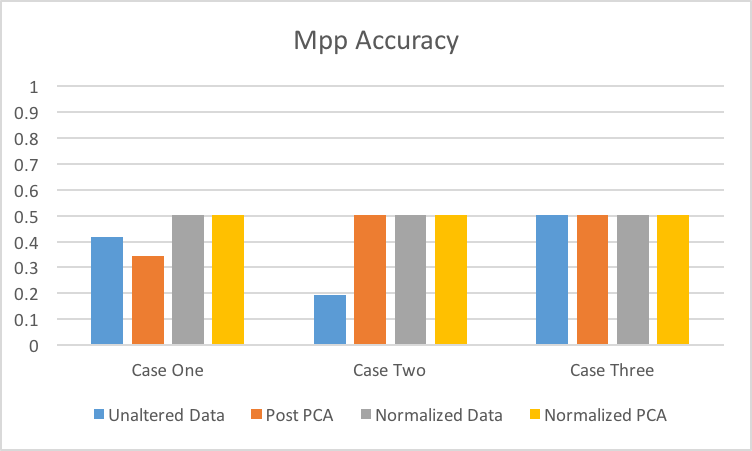
\includegraphics[width = 4.5in]{images/mpp-results}}

\paragraph{kNN}

\centerline{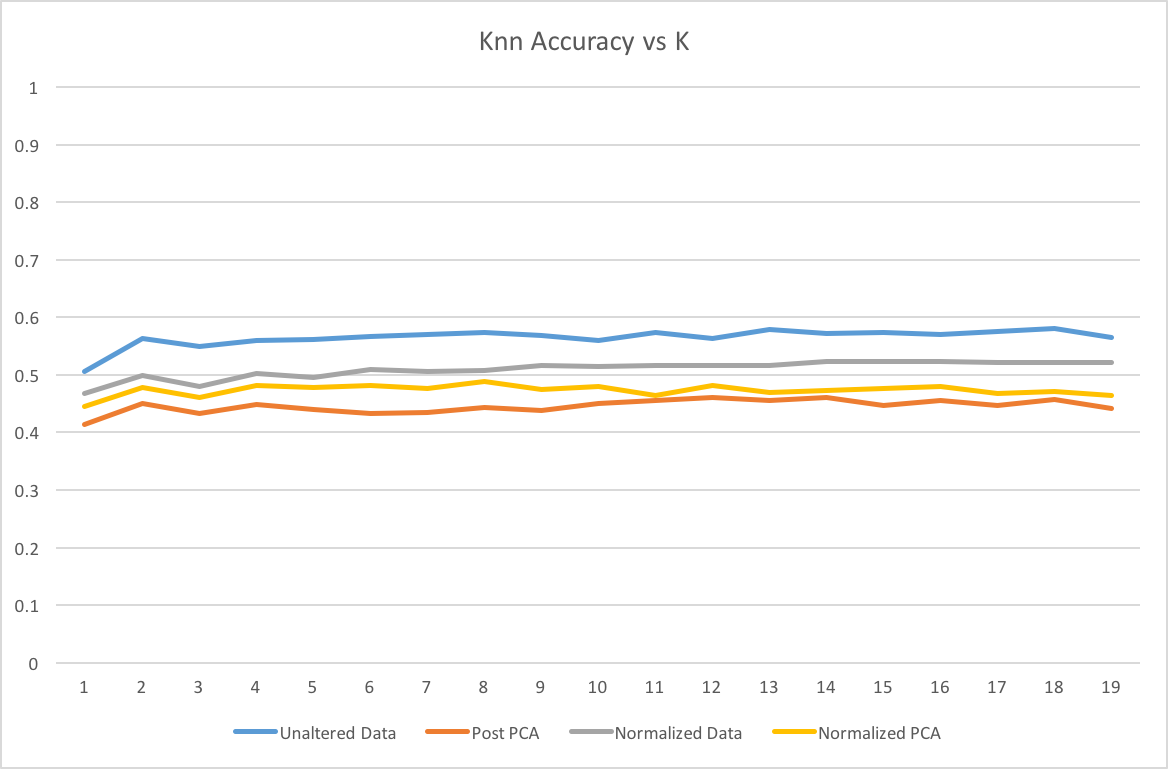
\includegraphics[width = 4.5in]{images/knn-results}}

\paragraph{BPNN}

\centerline{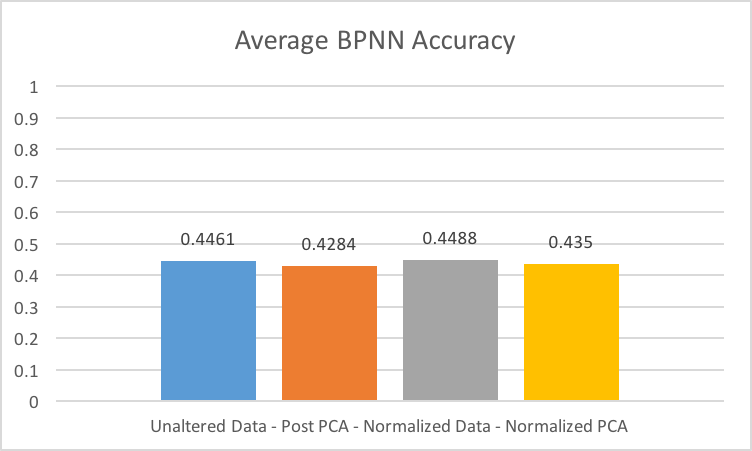
\includegraphics[width = 4.5in]{images/bpnn-results}}

\paragraph{Decision Tree}
The Decision tree algorithm was actually able to classify with an accuracy of one hundred percent when run on the testing set. The algorithm simply ran through each of the hands and had a node that decided for each of the groups since each group is defined in such a way that is known before hand and has to be a certain combination of the cards. This lead the algorithm to be very fast as well since it only goes through the data set one time to classify each hand.



\paragraph{K-means}

\centerline{\includegraphics[width = 4.5in]{../flowers}}

\paragraph{Winner-Take-All}
\paragraph{Kohonen Maps}

\centerline{\includegraphics[width = 4.5in]{../flowers}}
The original image \textit{flowers.ppm} is displayed above. All experiments
are performed on this image. The first expiriment is the kmeans clustering
of colors in \textit{flowers.png}. The resulting images can be seen on the following page. To generate these images k-means clustering was performed with [1, 2, 4, 8, 16
, 32, 64, 128, 256] clusters respectively.

\newpage
\centerline{
\includegraphics[width = 2in]{../kmeans/flowers_kmeans_1}
\includegraphics[width = 2in]{../kmeans/flowers_kmeans_2}
\includegraphics[width = 2in]{../kmeans/flowers_kmeans_4}}
\centerline{
\includegraphics[width = 2in]{../kmeans/flowers_kmeans_8}
\includegraphics[width = 2in]{../kmeans/flowers_kmeans_16}
\includegraphics[width = 2in]{../kmeans/flowers_kmeans_32}}
\centerline{
\includegraphics[width = 2in]{../kmeans/flowers_kmeans_64}
\includegraphics[width = 2in]{../kmeans/flowers_kmeans_128}
\includegraphics[width = 2in]{../kmeans/flowers_kmeans_256}}
The k-means images are seen above. The visual differences on these images are 
easy to see for the first couple images but by k=16 it becomes harder to find 
difference between the original image and the processed image. A list of the 
colors included in the each of these images is found in the apendix.
\newpage


%-----------------------------Evaluation------------------------
\section*{Evaluation}
\paragraph{}
Evalution was performed using 10-fold cross-validation for the kNN classifier.
Evaluation is performed in evaluation.py using standard Python language, with the support of
the math, random, numpy, and subprocess libraries.  This script performes the m-fold
cross-validation algorithm by dividing the dataset into m disjoint sets and iterates over them
using the 'leave-one-out' methodology, where one set is preserved as the testing (or validaiton)
set and the remaining m-1 sets are combined to become the new training set.  Normalization is
performed anew on each of the m iterations for the training and testing sets separately.
\newline
\newline
\centerline{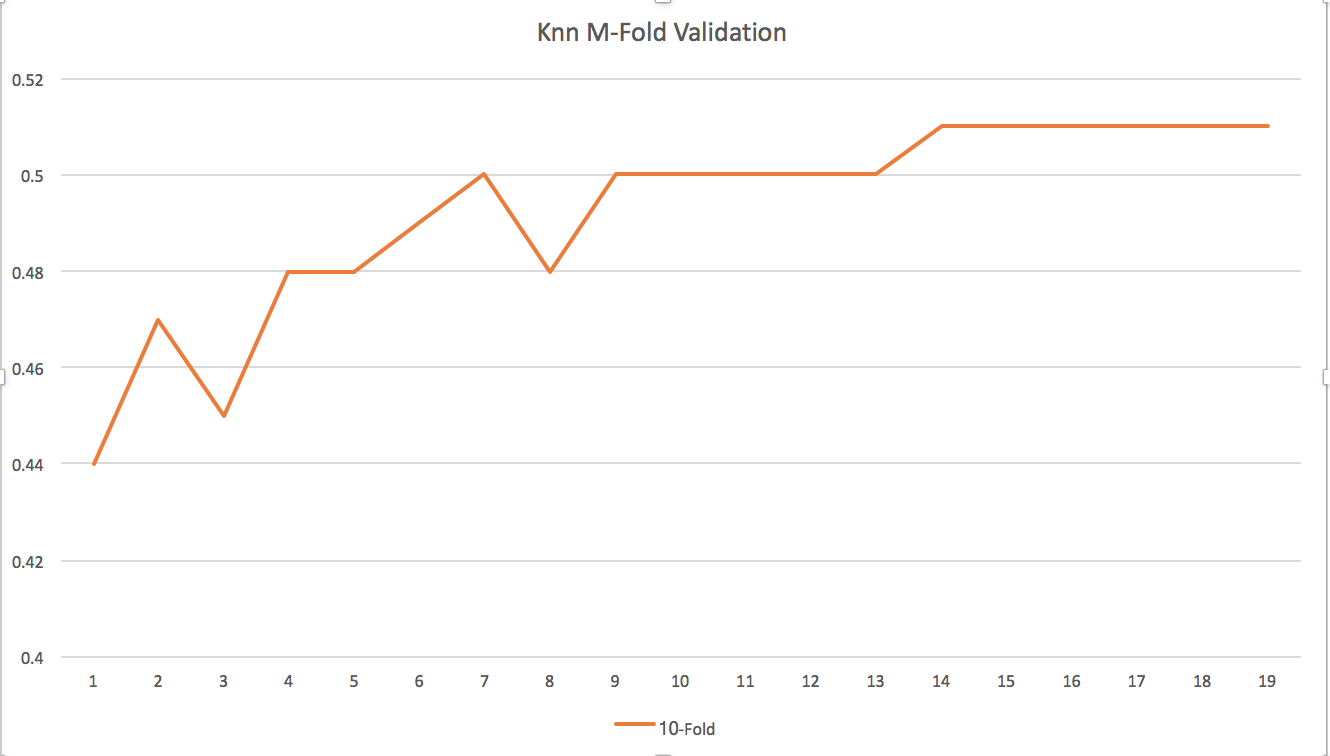
\includegraphics[width = 4.5in]{images/KNN_MFOLD2.png}}
\newline
\newline
kNN with 10-fold validation has a similar profile to the previous kNN trials performed with
generally lower accuracy due to near complete mitigation of training/testing cycle bias.
\newpage


%-----------------------------Discussion------------------------
\section*{Discussion}
\paragraph{}
This lab was very interesting to perform. Using python was a good
choice because it greatly simplified the k-means part of the lab.
The lab certainly increased my understanding of clustering algorithms 
and gave me greater insight to how and why they are used. The whole
concept of unsupervised learning is very interesting and it was fascinating
to see it in action here.
\newpage


%-----------------------------Reference------------------------
\section*{Discussion}
\paragraph{}
This lab was very interesting to perform. Using python was a good
choice because it greatly simplified the k-means part of the lab.
The lab certainly increased my understanding of clustering algorithms 
and gave me greater insight to how and why they are used. The whole
concept of unsupervised learning is very interesting and it was fascinating
to see it in action here.
\newpage


%----------------------------Appendix-----------------------------
\appendix
\section*{Appendix}
\subsection*{normalize.py}
\lstinputlisting[language=Python,numbers=left]{../normalize.py}
\newpage
\subsection*{mpp.py}
\lstinputlisting[language=Python,numbers=left]{../mpp.py}
\newpage
\subsection*{knn.py}
\lstinputlisting[language=Python,numbers=left]{../knn.py}
\newpage
\subsection*{backprop.py}
\lstinputlisting[language=Python,numbers=left]{../backprop.py}
\newpage
\subsection*{dtree.py}
\verbatiminput{../dtree.py}
\newpage
\subsection*{kmeans.c}
\verbatiminput{../kmeans.c}
\newpage
\subsection*{wta.c}
\lstinputlisting[language=Python,numbers=left]{../wta.c}
\newpage
\subsection*{kohonen.c}
\lstinputlisting[language=Python,numbers=left]{../kohonen.c}
\newpage
\subsection*{evaluation.py}
\lstinputlisting[language=Python,numbers=left]{../evaluation.py}
\newpage

\end{document}
